\documentclass{beamer}
% Try the class options [notes], [notes=only], [trans], [handout],
% [red], [compress], [draft] and see what happens!

% \usepackage{definitions}
\usepackage[british]{babel}

%% tikz tricks
% \tikzset{onslide/.code args={<#1>#2}{%
%   \only<#1>{\pgfkeysalso{#2}} 
% }}

\pdfinfo{
        /Title (cim)
        /Creator (LaTeX)
        /Producer (pdflatex)
        /Author (szerzo)
        /CreationDate (datum)
	/Subject (tema)
}


\mode<article> % only for the article version
{
  \usepackage{fullpage}
  \usepackage{hyperref}
}
\mode<presentation>
{
  \usetheme[left,width=0.65in,height=0.55in]{Kolozsvar}
  \setbeamercovered{transparent}
  \setbeamertemplate{navigation symbols}{}
  \setbeamertemplate{footline}%
     {\vspace*{-1.4em}\hspace*{0.66in}\textbf{\insertframenumber/\inserttotalframenumber}\newline\vspace*{0.4em}}
		\setbeamerfont{block title}{size=\larger} % RELSIZE -- html-sizes 
		\usefonttheme{professionalfonts}
		\setbeamercolor{math text}{fg=green!30!red!30!brown}
		\setbeamercolor{normal text in math text}{parent=math text}
}

\setbeamercovered{dynamic}

% The following info should normally be given in you main file:
\title[Main]{Automated Dental Disease Identification: Image Recognition-Based Approach for Advancing Dental Diagnostic Capabilities}
%
\author{Botond Biró, Hunor Ördög, Norbert R. Pap}
%
\institute[UBB Cluj-Napoca]{
  Department of Mathematics and Informatics\\
  Babe{\c{s}}--Bolyai University, Cluj-Napoca}
%
\date{March 2024}


\begin{document}

\frame{\maketitle}

\mode<presentation>
{
	\begin{frame}
	  \frametitle{Talk structure}
	\tableofcontents
	\end{frame} 

	\AtBeginSection[]
	{
  	\begin{frame}<beamer>{Contents}
    	\tableofcontents[currentsection,currentsubsection,hideothersubsections]
  	\end{frame}
	}
}

\section[Introduction]{Introduction}

\begin{frame}{Introduction}
	\begin{itemize}
		\vfill
		\item \textbf{Traditional method limitations}:
		\begin{itemize}
			\item Involves time constraints
			\item Prone to subjective interpretation
		\end{itemize}
		\vfill
		\item AI-driven approach
		\vfill
		\item \textbf{Algorithm}:
		\begin{itemize}
			\item Analyzes X-ray images accurately
			\item Identifies various dental conditions including subtle deviations
		\end{itemize}
		\vfill
		\item Enhances the accuracy
		\vfill
		\item Reduces missed diagnoses
		\vfill
		\item Empowers predictive dental care
	\end{itemize}
\end{frame}

\section[Related work]{Related work}

\begin{frame}{Related work}
	\begin{itemize}
		\vfill
		\item \textbf{Deep Learning for Periapical Disease}:A deep learning algorithm outperformed some manual diagnostics\cite{endres2020development}
		\vfill
		\item \textbf{CNNs for Caries Detection}: Highlights the potential of CNNs as a valuable tool to assist dental professionals \cite{lee2018detection}
		\vfill
		\item \textbf{Optimizing CNN Architectures}:Uses advanced image analysis techniques to improve diagnostic accuracy in dental radiology \cite{chen2021dental}
		\vfill
		\item \textbf{Multitask Classification of Dental Disease}: Highlights the importance of using advanced machine learning techniques to automate disease classificasion tasks \cite{al2022detection}
	\end{itemize}
\end{frame}

\begin{frame}{Related work}
	\begin{itemize}
		\vfill
		\item \textbf{Expert Systems for Diagnosis}: Highlights the effectiveness of expert systems in providing accurate and reliable diagnoses \cite{setiabudi2017expert}
		\vfill
		\item \textbf{Hybrid Approach for Disease Detection}: Combines fuzzy logic and evolutionary strategies to improve accuracy in dental disease detection \cite{parewe2018dental}
	\end{itemize}
\end{frame}

\section[Materials and Methods]{Materials and Methods}

\begin{frame}{Dataset}
	\begin{itemize}
		\vfill
		\item \textbf{Dataset Overview}:
		\begin{itemize}
			\item 10,000 dental X-ray images
			\item Reputable sources
			\item Diseases included: caries, periodontal disease, malocclusions
			\item Partitioned into training sets(80\%) and test sets(20\%)
		\end{itemize}
		\vfill
		\item \textbf{Preprocessing}:
		\begin{itemize}
			\item Standardize the data, optimize its suitability
			\item Steps:
			\begin{enumerate}
				\item Normalization
				\item Noise reduction
				\item Contrast enhancement
			\end{enumerate}
		\end{itemize}
	\end{itemize}
\end{frame}

\begin{frame}{Radiographs depicting various dental diseases}
	\begin{figure}[!t]
		\centerline{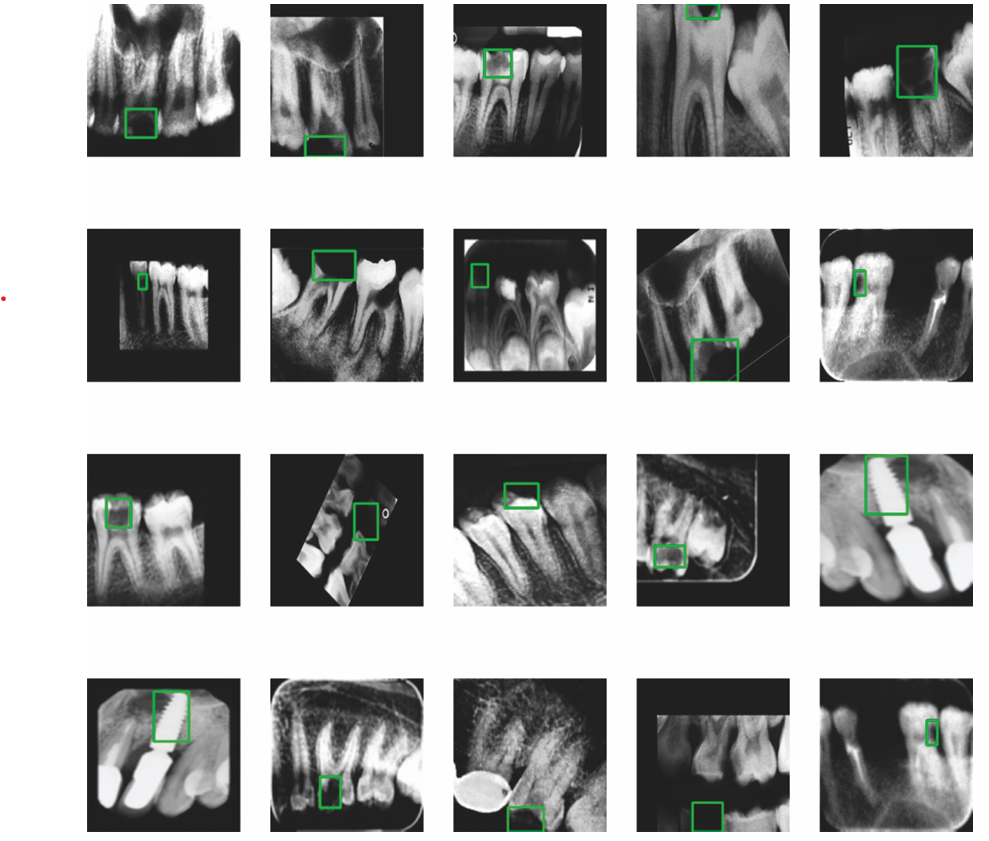
\includegraphics[width=0.9\textwidth]{../ss-teeth-full.png}}
	\end{figure}
\end{frame}

\begin{frame}{Proposed Methodology}
	\begin{itemize}
		\vfill
		\item \textbf{Utilization of CNNs and Attention Mechanisms}: Unravels subtle disease signatures in dental X-rays efficiently	
		\vfill 
		\item \textbf{Image augmentation}: Utilizes techniques: rotation, flipping, noise reduction, contrast enhancement
		\vfill 
		\item \textbf{Feature Extraction}: Captures meaningful information
		\vfill
		\item \textbf{Training and Optimization}:
		\begin{itemize}
			\item Refines diagnostic acumen
			\item Ensures exposure to diverse pathologies
			\item Fine-tunes internal parameters
		\end{itemize}
	\end{itemize}
\end{frame}

\begin{frame}{Data Augmentation}
  	\begin{itemize}
		\vfill
		\item \textbf{Augmentation pipeline}: Simulates real-world acquisition conditions(scaling, ratation, translation) and introduces controlled variations
		\vfill
		\item \textbf{Simulated Degradations}:
		\begin{itemize}
			\item Gaussian blur to mimic potential issues arising from motion blur
			\item Gaussian noise to simulate the presence of random noice to the pixel intensities
		\end{itemize}
		\vfill
		\item \textbf{Enhancing Diversity and Breadth}: Covers the range of potential inconsistencies encountered in real-world dental X-ray images
		\vfill
		\item \textbf{Addressing Overfitting}
	\end{itemize}
\end{frame}

\begin{frame}{Preprocessing of the Image Dataset}
	\begin{itemize}
		\vfill
		\item \textbf{Normalization and Resizing}:
		\begin{itemize}
			\item Standardizes pixel intensities
			\item Ensures consistent dimensions
		\end{itemize}
		\vfill
		\item \textbf{Specialized Encoding}:
		\begin{itemize}
			\item Handles categorical data, such as disease labels
			\item Implements Label and One-Hot Encoding
		\end{itemize}
		\vfill
		\item \textbf{Bridge to Analytics}: Prepares data for feature extraction and disease classification
	\end{itemize}
\end{frame}

\begin{frame}{Construction of the Multi-Output Model: A Deep Learning Approach}
	\begin{itemize}
		\vfill
		\item \textbf{Transfer Learning Integration}: Utilizes pre-trained CNNs for foundational knowledge
		\vfill
		\item \textbf{Convolutional Layers}:Extracts hierarchical features from X-ray images and identify complex disease signatures via filters
		\vfill
		\item \textbf{Max-Pooling Layers}:
		\begin{itemize}
			\item Reduces dimensionality while preserving features
			\item Enhances efficiency and prevent overfitting
		\end{itemize} 
		\vfill
		\item \textbf{Dropout Layers}: Introduces a controlled element of randomness
		\vfill
		\item \textbf{Activation Functions}: Introduces non-linearity for complex pattern learning
		\vfill
		\item \textbf{Fully-Connected Layers}: Output layer enables probability-based identification
	\end{itemize}
\end{frame}

\begin{frame}{Flowchart of the proposed work}
	\begin{figure}[!t]
		\centerline{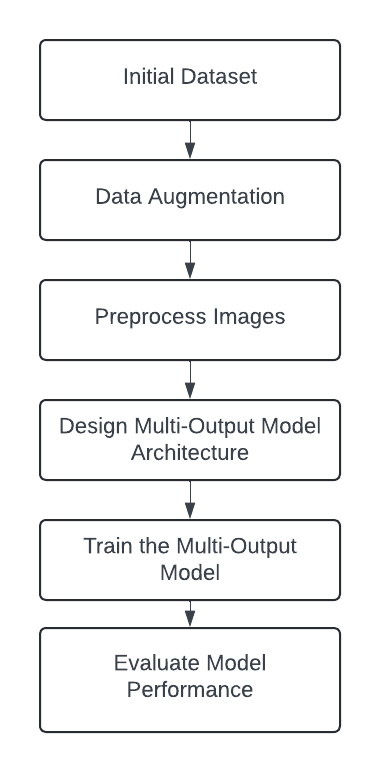
\includegraphics[width=0.55\textwidth]{../flowchart.png}}
	\end{figure}
\end{frame}

\section[Results and Discussion]{Results and Discussion}

\begin{frame}{Model Accuracy}
	\begin{itemize}
		\vfill
		\item \textbf{Model Evaluation}: Tested on 20\% of dataset and achieved over 97\% average accuracy
		\begin{table}[h]
			\centering
			\begin{tabular}{|c|c|c|}
				\hline
				\textbf{Diseases}      & \textbf{Occurrence} & \textbf{Accuracy (\%)} \\
				\hline
				Tooth Decay (Caries)   & 250                 & 97.6                   \\
				Gingivitis             & 150                 & 97.8                   \\
				Periodontitis          & 120                 & 97.7                   \\
				Bad Breath (Halitosis) & 100                 & 97.2                   \\
				Tooth Sensitivity      & 50                  & 97.9                   \\
				Oral Cancer            & 200                 & 97.3                   \\
				Dental Abscess         & 180                 & 97.5                   \\
				Dental Erosion         & 70                  & 97.1                   \\
				Bruxism                & 100                 & 97.4                   \\
				Malocclusion           & 200                 & 97.0                   \\
				Pulpitis               & 180                 & 97.6                   \\
				No disease             & 400                 & 98.3                   \\
				\hline
			\end{tabular}
		\end{table}
	\end{itemize}
\end{frame}

\begin{frame}{Implications and Future Directions}
	\begin{itemize}
		\vfill
		\item \textbf{Augmenting Diagnostic Capabilities}:
		\begin{itemize}
			\item Facilites early detection and intervention
			\item Improves treatment outcomes
		\end{itemize} 
		\vfill
		\item \textbf{Revolutionizing Dental Diagnostics}: 
		\begin{itemize}
			\item Leverages deep learning and diverse dataset
			\item Potential for more effective patient care
		\end{itemize} 
		\vfill
		\item \textbf{Opportunities for Improvement}:
		\begin{itemize}
			\item Dataset Expansion: Includes broader clinical scenarios and demographics
			\item Advances in Deep Learning: Optimizes methodology for better performance
		\end{itemize} 
	\end{itemize}
\end{frame}

\section[Conclusion]{Conclusion}
\begin{frame}{Conclusion}
	\begin{itemize}
		\vfill
		\item \textbf{Significance}: Represents a significant leap in AI integration into dental practice
		\vfill
		\item Enables dentists to deliver more efficient, accurate and preventative dental care
		\vfill
		\item Exceptional accuracy in identifying a wide range of dental conditions
	\end{itemize}
\end{frame}

\section[Questions]{Questions}
\begin{frame}{Questions}
\end{frame}

\section{References}
\begin{frame}[allowframebreaks]{References}
	\nocite{*}
    \bibliographystyle{unsrt}
    \bibliography{references}
\end{frame}

\end{document}
